\documentclass{standalone}
\usepackage{pgfplots}
\usepackage{tikz}
\pgfplotsset{compat=newest}
\usetikzlibrary{calc,intersections}  
\usetikzlibrary{arrows,shapes,positioning}
\usetikzlibrary{decorations.markings}
\usetikzlibrary{spy,shadows}
\tikzset{spy using overlaysshadow/.style={
		spy scope={#1,
			every spy on node/.style={
				circle,
				fill, fill opacity=0.2, text opacity=1
			},
			every spy in node/.style={
				circle, circular drop shadow,
				fill=white, draw, ultra thick, cap=round
			}
		}
	}
}
\begin{document}
\tikzset{
	name path global/.append code={%
		\csname tikz@addmode\endcsname{%
			\pgfgetpath\tmp%
			\expandafter\global\expandafter\let\csname tikz@intersect@path@name@#1\endcsname=\tmp%
		}%
	}%
}  
\begin{tikzpicture}[spy using overlaysshadow={
	magnification=6, 
	size=1.5cm, 
	connect spies}
]
\tikzstyle directed=[decoration={markings,
		mark=at position .5 with {\arrow{stealth}}}]
\begin{axis}
[
width=7.2cm,
height=6cm,
name=firstaxis, 
domain=-0.5:11, 
xmin=-0.5, xmax=11, 
ymin=-5, ymax=220, 
enlargelimits=false,
axis line style={draw=none},
ticks=none,
scale only axis
]
\addplot[name path global=voltage,smooth,blue,line width=0.5pt]{(10-x)/0.05};
\addplot[name path global=R,smooth,red,line width=0.5pt]{x^3/5};

% Draw intersections points
%\fill [black, name intersections={of=voltage and R}] (intersection-1) circle [radius=1pt];  
%\def \n {10};
%\def \Z0 {0.01};
%\foreach \s in {1,...,\n}
%{
%    \addplot [-stealth] coordinates {(\s, 2)(\s, 200)};
%}	
%%%%%%%%%%%%%%%%%%%%%%%%%%
\node[right, align=left]
at (axis cs:0.909,181.818) {1};
\addplot [ draw=none, mark size=0.5pt, mark=*, mark options={solid, fill=black, black}]
table[row sep=crcr]{%
	0.909090909090909	181.818181818182\\
};


\addplot [postaction={decorate},directed,color=gray, dotted, line width=0.4pt]
table[row sep=crcr]{%
	0	0\\
	0.909090909090909	181.818181818182\\
};


\node[right, align=left]
at (axis cs:1.812,1.19) {2};
\addplot [ draw=none, mark size=0.5pt, mark=*, mark options={solid, fill=black, black}]
table[row sep=crcr]{%
	1.8122301317607	1.19033728422266\\
};


\addplot [postaction={decorate},directed,color=gray, dotted, line width=0.4pt]
table[row sep=crcr]{%
	0.909090909090909	181.818181818182\\
	1.8122301317607	1.19033728422266\\
};


\node[right, align=left]
at (axis cs:2.551,148.977) {3};
\addplot [ draw=none, mark size=0.5pt, mark=*, mark options={solid, fill=black, black}]
table[row sep=crcr]{%
	2.55116222303599	148.97675553928\\
};


\addplot [postaction={decorate},directed,color=gray, dotted, line width=0.4pt]
table[row sep=crcr]{%
	1.8122301317607	1.19033728422266\\
	2.55116222303599	148.97675553928\\
};


\node[right, align=left]
at (axis cs:4.738,21.273) {4};
\addplot [ draw=none, mark size=0.5pt, mark=*, mark options={solid, fill=black, black}]
table[row sep=crcr]{%
	4.73803652441242	21.2728270123115\\
};


\addplot [postaction={decorate},directed,color=gray, dotted, line width=0.4pt]
table[row sep=crcr]{%
	2.55116222303599	148.97675553928\\
	4.73803652441242	21.2728270123115\\
};


\node[right, align=left]
at (axis cs:5.12,97.606) {5};
\addplot [ draw=none, mark size=0.5pt, mark=*, mark options={solid, fill=black, black}]
table[row sep=crcr]{%
	5.11970217213715	97.605956557257\\
};


\addplot [postaction={decorate},directed,color=gray, dotted, line width=0.4pt]
table[row sep=crcr]{%
	4.73803652441242	21.2728270123115\\
	5.11970217213715	97.605956557257\\
};


\node[right, align=left]
at (axis cs:6.857,64.483) {6};
\addplot [ draw=none, mark size=0.1pt, mark=*, mark options={solid, fill=black, black}]
table[row sep=crcr]{%
	6.85707758575988	64.4832897606222\\
};


\addplot [postaction={decorate},directed,color=gray, dotted, line width=0.4pt]
table[row sep=crcr]{%
	5.11970217213715	97.605956557257\\
	6.85707758575988	64.4832897606222\\
};


%\node[right, align=left]
%at (axis cs:6.85,63.006) {7};
\addplot [ draw=none, mark size=0.1pt, mark=*, mark options={solid, fill=black, black}]
table[row sep=crcr]{%
	6.84969194268797	63.0061611462405\\
};


\addplot [color=black, line width=0.1pt]
table[row sep=crcr]{%
	6.85707758575988	64.4832897606222\\
	6.84969194268797	63.0061611462405\\
};


\addplot [ draw=none, mark size=0.1pt, mark=*, mark options={solid, fill=black, black}]
table[row sep=crcr]{%
	6.81558791950714	63.3198633679237\\
};


\addplot [color=black, line width=0.1pt]
table[row sep=crcr]{%
	6.84969194268797	63.0061611462405\\
	6.81558791950714	63.3198633679237\\
};


\addplot [ draw=none, mark size=0.1pt, mark=*, mark options={solid, fill=black, black}]
table[row sep=crcr]{%
	6.81726236606138	63.6547526787723\\
};


\addplot [color=black, line width=0.1pt]
table[row sep=crcr]{%
	6.81558791950714	63.3198633679237\\
	6.81726236606138	63.6547526787723\\
};


\addplot [ draw=none, mark size=0.1pt, mark=*, mark options={solid, fill=black, black}]
table[row sep=crcr]{%
	6.8249986864983	63.5825164147689\\
};


\addplot [color=black, line width=0.1pt]
table[row sep=crcr]{%
	6.81726236606138	63.6547526787723\\
	6.8249986864983	63.5825164147689\\
};


\addplot [ draw=none, mark size=0.1pt, mark=*, mark options={solid, fill=black, black}]
table[row sep=crcr]{%
	6.82462373129496	63.5075253741008\\
};


\addplot [color=black, line width=0.1pt]
table[row sep=crcr]{%
	6.8249986864983	63.5825164147689\\
	6.82462373129496	63.5075253741008\\
};


\addplot [ draw=none, mark size=0.1pt, mark=*, mark options={solid, fill=black, black}]
table[row sep=crcr]{%
	6.82289157314363	63.5236442228578\\
};


\addplot [color=black, line width=0.1pt]
table[row sep=crcr]{%
	6.82462373129496	63.5075253741008\\
	6.82289157314363	63.5236442228578\\
};


\addplot [ draw=none, mark size=0.1pt, mark=*, mark options={solid, fill=black, black}]
table[row sep=crcr]{%
	6.82297577457213	63.5404845085574\\
};


\addplot [color=black, line width=0.1pt]
table[row sep=crcr]{%
	6.82289157314363	63.5236442228578\\
	6.82297577457213	63.5404845085574\\
};


\addplot [ draw=none, mark size=0.1pt, mark=*, mark options={solid, fill=black, black}]
table[row sep=crcr]{%
	6.82336476594651	63.5368619395766\\
};


\addplot [color=black, line width=0.1pt]
table[row sep=crcr]{%
	6.82297577457213	63.5404845085574\\
	6.82336476594651	63.5368619395766\\
};


\addplot [ draw=none, mark size=0.1pt, mark=*, mark options={solid, fill=black, black}]
table[row sep=crcr]{%
	6.82334586931694	63.5330826136613\\
};


\addplot [color=black, line width=0.1pt]
table[row sep=crcr]{%
	6.82336476594651	63.5368619395766\\
	6.82334586931694	63.5330826136613\\
};


\addplot [ draw=none, mark size=0.1pt, mark=*, mark options={solid, fill=black, black}]
table[row sep=crcr]{%
	6.82325857176017	63.5338954528449\\
};


\addplot [color=black, line width=0.1pt]
table[row sep=crcr]{%
	6.82334586931694	63.5330826136613\\
	6.82325857176017	63.5338954528449\\
};


\addplot [ draw=none, mark size=0.1pt, mark=*, mark options={solid, fill=black, black}]
table[row sep=crcr]{%
	6.82326281317813	63.5347437364375\\
};


\addplot [color=black, line width=0.1pt]
table[row sep=crcr]{%
	6.82325857176017	63.5338954528449\\
	6.82326281317813	63.5347437364375\\
};


\addplot [ draw=none, mark size=0.1pt, mark=*, mark options={solid, fill=black, black}]
table[row sep=crcr]{%
	6.82328240746368	63.5345612844427\\
};


\addplot [color=black, line width=0.1pt]
table[row sep=crcr]{%
	6.82326281317813	63.5347437364375\\
	6.82328240746368	63.5345612844427\\
};


\addplot [ draw=none, mark size=0.1pt, mark=*, mark options={solid, fill=black, black}]
table[row sep=crcr]{%
	6.82328145549225	63.5343708901551\\
};


\addplot [color=black, line width=0.1pt]
table[row sep=crcr]{%
	6.82328240746368	63.5345612844427\\
	6.82328145549225	63.5343708901551\\
};


\addplot [ draw=none, mark size=0.1pt, mark=*, mark options={solid, fill=black, black}]
table[row sep=crcr]{%
	6.82327705762475	63.5344118405023\\
};


\addplot [color=black, line width=0.1pt]
table[row sep=crcr]{%
	6.82328145549225	63.5343708901551\\
	6.82327705762475	63.5344118405023\\
};
%%%%%%%%%%%%%%%%%%%%%%%
\addplot [-stealth,color=black,line width=0.8pt]
table[row sep=crcr]{%
	0	-50\\
	0	220\\
};

\addplot [-stealth,color=black,line width=0.8pt]
table[row sep=crcr]{%
	-1	0\\
	11	0\\
};
\fill [black] (axis cs:0,0)circle[radius=1pt];
\node [above] at (axis cs:10.5,0){U};
\node [right] at (axis cs:0,210){I};
%\node  at (axis cs:0.2,7){O};	
\spy [red] on (4.6,1.9) in node [left] at (4.5,3.7);
\node[right, align=left]
at (axis cs:0,6) {0};
\end{axis}
	
\end{tikzpicture}
	
\end{document}
